\section{Komponentenschnittstellen}

%3.1 Datentypen
\subsection{\textit{Datentypen}}
Die in Abbildung \ref{KomponentenschnittstellenDiagramm} dargestellten Datentypen werden von den Schnittstellen der eingeführten Komponenten verwendet. 

Die Aufgabe des Datentyp SensorData ist es primär, die Koordination mit dem Server zu unterstützen, um festzustellen, inwieweit eine Zielposition gut erreicht werden kann. Dazu besitzt er als Attribute die Orientierungsrichtung im Koordinatensystem, den Batteriestatus, seine Position in den räumlichen Koordinaten und zuletzt die mit einem eigenen Datentyp versehene Destination. Wird dem Roboter nun eine neue Task zugewiesen, erhält er damit genau diesen Datentyp Destination und die damit verbundene position des Patienten. Mit dem Attribut speed kann der Server außerdem genau bestimmen, mit welcher Geschwindigkeit der Roboter den Patienten anlaufen soll – also die Wichtigkeit des Einsatzes bestimmen.

	
	\begin{figure}[H]
		\centering
		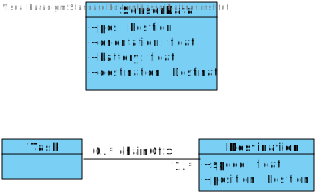
\includegraphics[width=0.75\textwidth]{img/0-Entwurf-3.svg}
		\caption{Datentypen, die in Komponentenschnittstellen verwendet werden}
		\label{KomponentenschnittstellenDiagramm}
	\end{figure}
	\pagebreak

%3.2 Interfaces
\subsection{\textit{Interfaces}}
	%3.2.1 ISensorData
	\subsubsection{\textit{ISensorData}}
	Dieses \textit{Interface} wird vom \textit{Robot} angeboten, um dem Server alle Sensordaten zu senden. Der Server kann anhand diesen jederzeit feststellen, in welchem Zustand sich der \textit{Robot} befindet um diesem dann eine \textit{Task} zuzuweisen.
	\begin{figure}[H]
	\centering
	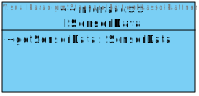
\includegraphics[width=0.25\textwidth]{img/1-Entwurf-3-1_ISensorData}
	\caption{\textit{Interface} ISensorData}
	\label{ISensorData}
	\end{figure}
	
	%3.2.2 ITask
	\subsubsection{\textit{ITask}}
	Dieses \textit{Interface} wird vom \textit{Robot} angeboten, um Tasks zu erhalten. Der Server kann somit ohne Probleme \textit{Tasks} dem \textit{Robot} zuweisen. Hierbei findet eine Unidirektionale Kommunikation zwischen Server und Robot statt.
	\begin{figure}[H]
	\centering
	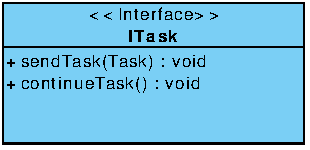
\includegraphics[width=0.25\textwidth]{img/1-Entwurf-3-1_ITask}
	\caption{\textit{Interface} ITask}
	\label{ITask}
	\end{figure}
